\chapter{Hypothesis testing}
\label{hypothesisTesting}
\label{sectionHypothesisTesting}

\section{Introduction}
%__________________
%\section{Hypothesis testing}
\label{hypothesisTesting}

\index{hypothesis testing|(}

In this Chapter we use statistics to make conclusions on parameters. 
In Chapter~\ref{sectionConfidenceIntervals} we constructed a range of values which we stated captured the mean with a certain level of confidence.
In this chapter we will learn techniques to quantify the strength of a conclusion using probability.


The mathematical background behind a hypothesis test starts with a decision rule which is
something that is used to decide on a conclusion to make regarding the value of a parameter based on the result of a test.
A \emph{test statistic} is a value calculated using sample data as well as a
value from a status quo belief. 
Test statists are derived using a decision rule as well as something called the
likelihood ratio test.
These topics are more suited for advanced undergraduate of graduate courses in mathematical statistics but 
me mention them so that the reader is aware about the rigorous mathematical framework behind hypothesis tests. 

For an introductory course we will skip the mathematical derivation of a hypothesis test and
get right into the procedure of conducting them.
This makes the process of hypothesis testing somewhat algorithmic to some extent.
There are several steps involved in performing a hypothesis test.
We will list each of the steps involved and discuss each of them in more detail.


\begin{enumerate}
\item	State the null and alternative hypothesis
\item	Find the appropriate test statistic
\item	Find the p-value associated with the hypothesis test
\item	Compare the p-value to a level of significance $(\alpha)$
\item	Make a conclusion
\end{enumerate}

%The order of the steps in which hypothesis tests are done is always the same as those mentioned above. 
The hypothesis testing framework is a very general tool, and we often use it without a second thought. If a person makes a somewhat unbelievable claim, we are initially skeptical. However, if there is sufficient evidence that supports the claim, we set aside our skepticism and reject the null hypothesis in favour of the alternative. The hallmarks of hypothesis testing are also found in the US court system. 
In {\color{red}{Chapters ???}} we will learn about hypothesis tests on different parameters
however the procedure involved is the same.




\vfill


\subsection{State the null and alternative hypothesis}
\label{sectionStateNullAndAlternative}

The first step in hypothesis testing is to state the null and alternative hypothesis.
The  \term{null hypothesis} is the conservative or skeptical belief
and the  \term{alternative hypothesis} is the claimed belief.
The alternative is usually a researchers' belief.
The null hypothesis is represented by $H_{0}$ and the 
alternative hypothesis is represented by $H_{a}$.\footnote{Some textbooks might represent the alternative hypothesis by $H_1$ rather than $H_a$. This is also acceptable standard notation. However we will use 
$H_a$ to represent the alternative hypothesis.}


\begin{termBox}{\tBoxTitle{Null and alternative hypotheses}
%{\small 

\begin{tabular}{l c l}
$H_0$	& : 	& 	Null hypothesis	\\
	 	& 	&	Represents either a skeptical or conservative perspective on a claim to\\
		&	&	 be tested. \\
\hfill\\
$H_a$ 	& : 	& 	Alternative hypothesis\\
		&  	& 	Represents an alternative claim under consideration and is often \\
		&	&	represented by a range of possible parameter values.
\end{tabular} \vspace{2mm} }
\end{termBox}

When we stated that the null null hypothesis represents the conservative belief;
by this we mean that it represents the safe belief.
For example, during the development of a pharmaceutical drug the conservative belief
is to believe that the drug has no affect and does not work. 
%This is because it is safer to keep a drug out of a market rather than believe that it does work 
%when it actually does not and risk 

In the hypothesis testing framework we start by assuming that $H_{0}$ is true 
(since it is the safe belief) and then we continue to find evidence either supporting 
$H_{0}$ or against $H_{0}$.

Suppose $\gamma$ is the parameter we are interested in and $\gamma_{0}$ is the hypothesized value of 
$\gamma$ under the null hypothesis. 
We are being very general here and $\gamma$ can represent the population mean$\mu$ or
the population proportion $p$ is a difference of population means $\mu_1 - mu_2$ etc.
$\gamma_{0}$ is some numeric value $\gamma$ is supposed to equal under the null hypothesis.
There are 3 possible hypothesis tests we can perform on $\gamma$ and these are:\\

\begin{enumerate}
\item	$H_{0} = \gamma_{0}$ ~vs.~ $H_{a} > \gamma_{0}$	\label{onetailgreater}
\item	$H_{0} = \gamma_{0}$ ~vs.~ $H_{a} < \gamma_{0}$	\label{onetailless}
\item	$H_{0} = \gamma_{0}$ ~vs.~ $H_{a} \neq \gamma_{0}$	\label{twotail}
\end{enumerate}

We can only perform one of the hypothesis tests above at a time 
(i.e. we do not conduct all 3 hypothesis tests simultaneously).
Hypothesis tests~\ref{onetailgreater} and~\ref{onetailless} are called 
\term{one tailed tests} or \term{one sided tests}
and hypothesis test~\ref{twotail} is called the \term{two tailed test}
or \term{two sided test}.
These terms will become more familiar in {\color{red}{Chapter ???}}.



\begin{tipBox}{\tipBoxTitle{Always write the null hypothesis as an equality}
We will find it most useful if we always list the null hypothesis as an equality (e.g. $\mu = 7$) while the alternative always uses an inequality (e.g. $\mu\neq7$, $\mu>7$, or $\mu<7$).}
\end{tipBox}


The null hypothesis often represents a skeptical position or a perspective of no difference. The alternative hypothesis often represents a new perspective, such as the possibility that there has been a change. 



\subsection{Find the appropriate test statistic}
\label{sectionFindingAppropriateTestStat}

The test statistic that we calculate depends on the situation and the information available.
An estimator and the assumed parameter value under the null hypothesis is
used in the calculation of the test statistic.

\begin{termBox}{\tBoxTitle{Basic skeleton of a test statistic}
\vspace{-3mm}
\begin{align}
\text{test statistic}	& = 	\frac{(\text{an estimator}) - \bigg(\parbox{5.75cm}{\centering hypothesized value of the parameter under the null hypothesis}\bigg)}{(\text{Standard error of estimate})}\label{eqSkeletopTestStat}
\end{align}
\vspace{-3mm}
}
\end{termBox}


Compare~\vref{eqSkeletopTestStat} with
the basic skeleton of a confidence interval (i.e. \vref{tboxSkeletonOfCI})
and notice the similarities.
hypothesized value of the parameter under the null hypothesis refers to the numeric value of
$\gamma_0$ that was discussed in Chapter~\ref{sectionStateNullAndAlternative}.
So two things that the test statistic depend on are the data that is used to calculate the estimator
and $\gamma_0$.

The calculated test statistic follows a certain reference distribution.

\begin{termBox}{\tBoxTitle{Summary of reference distributions to use for hypothesis tests}

\begin{tabular}{l c l}
When $\sigma$ is known		&	$\longrightarrow$	&	estimator $\sim$ Z distribution		\\
When $\sigma$ is not known	&	$\longrightarrow$	&	estimator $\sim$ $t$ distribution	\\
For proportions				&	$\longrightarrow$	&	estimator $\sim$ Z distribution
\end{tabular}
}
\end{termBox}

We use the test statistic along with its reference distribution to calculate 
the p-value which is something we discuss in Chapter~\ref{sectionFindingPValue}.


\hfill\\

\subsection{Find the p-value}
\label{sectionFindingPValue}

The \term{p-value} is a way of quantifying the strength of the evidence against the null hypothesis and in favour of the alternative. 
The p-value depends on the the test statistic calculated (see Chapter~\ref{sectionFindingAppropriateTestStat})
and the alternative hypothesis (see Chapter~\ref{sectionStateNullAndAlternative}).
Formally the \emph{p-value} is a conditional probability.

\begin{termBox}{\tBoxTitle{p-value}
The p-value\index{hypothesis testing!p-value|textbf} 
is the probability of observing a test statistic at least as extreme as the one calculated with the sample data
collected purely by chance under the assumption that $H_0$ is true. 
}
\end{termBox}

%The \term{p-value}\index{hypothesis testing!p-value|textbf} is the probability of observing data at least as favorable to the alternative hypothesis as our current data set, if the null hypothesis is true. We typically use a summary statistic of the data, in this chapter the sample mean, to help compute the p-value and evaluate the hypotheses.}
It is important to note that we used the words ``at least as extreme'' and not just ``as extreme'' in the 
definition of the p-value in the text box above.
An alternate way to defining the p-value is that it is the probability of observing data at least as favourable to the alternative hypothesis as our current data set, if the null hypothesis is true. 
The estimator mentioned in Chapter~\ref{sectionFindingAppropriateTestStat} is 
used to be representative of the data.
%in this chapter the sample mean, to help compute the p-value and evaluate the hypotheses.

Also recall from Chapter~\ref{sectionFindingAppropriateTestStat} that the test static calculated with
\ref{eqSkeletopTestStat} follows a certain distribution.
The test statistic calculated for the hypothesis test is used along with the alternative hypothesis
to determine the p-value.
We illustrate this in Figure~\ref{} below.
Note that we are not being specific about the distribution used and the curve just represents
any valid reference distribution for the test statistic calculated. 
We use a bell-shaped curve in this figure because the only reference distributions that 
we cover in this text are the standard normal distribution and the $t$ distribution and both
of these are bell-shaped.

If we are conducting a one tailed test, the p-value is the area to the right of the test statistic
on the reference distribution if the alternative is that the parameter is greater than the hypothesized value.
This is illustrated in Figures~\ref{figHaGreater} and~\ref{figHaGreaterLargeTail} below.

\begin{figure}[H]
\begin{minipage}[b]{0.5\linewidth}
\centering
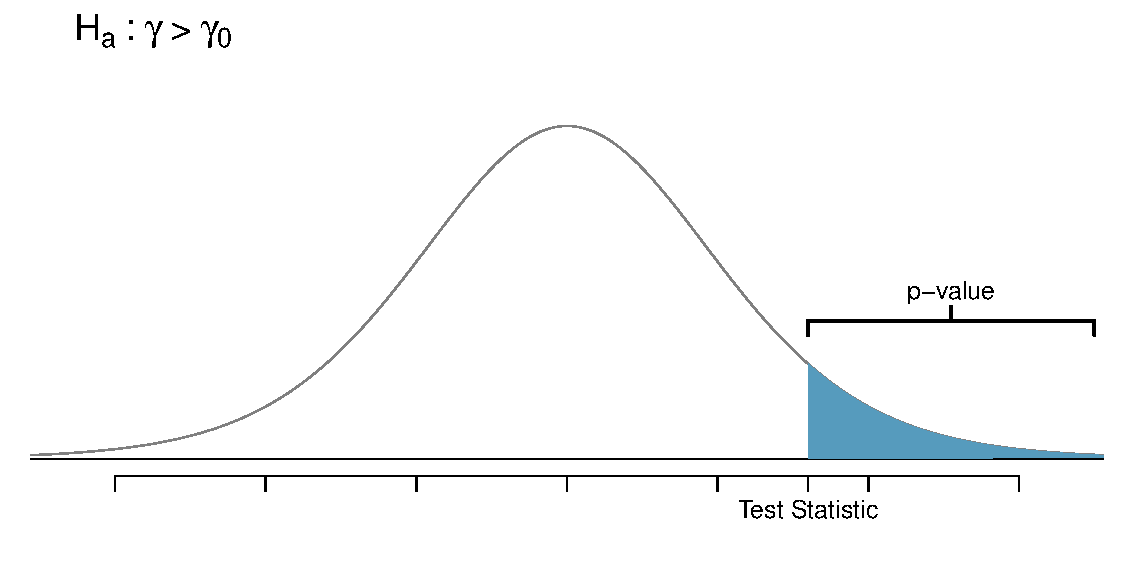
\includegraphics[width=\textwidth]{05-5/figures/pvalAlternaterGreaterThan/pvalAlternateGreaterThanSmallTail.pdf}
\captionsetup{width=0.9\textwidth}
\caption{Finding the p-value when $H_a : \gamma > \gamma_0$ }
\label{figHaGreater}
\end{minipage}
%\hspace{0.5cm}
\quad
\begin{minipage}[b]{0.5\linewidth}
\centering
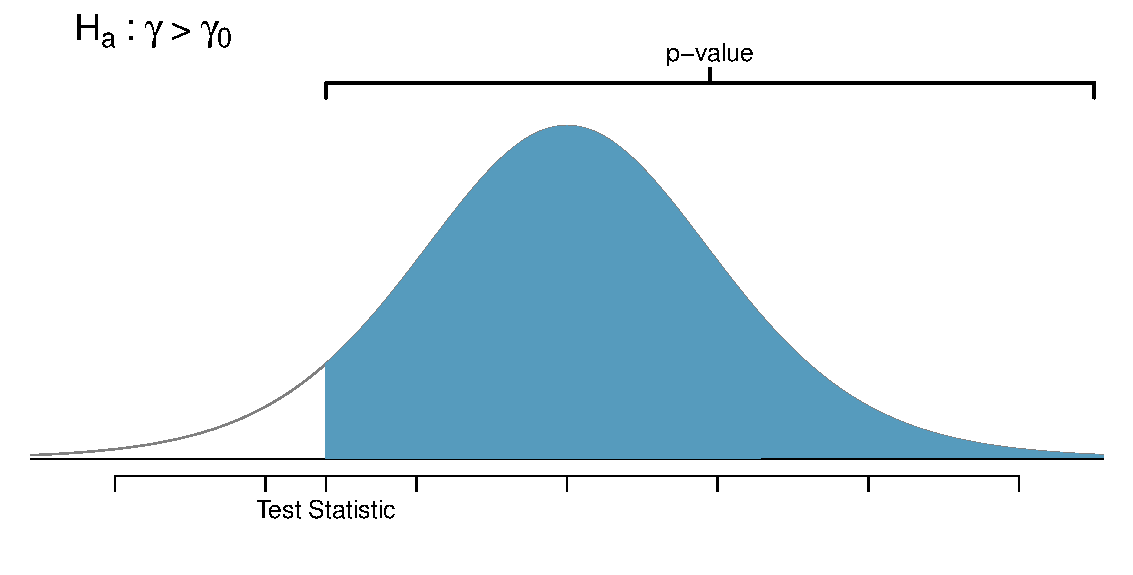
\includegraphics[width=\textwidth]{05-5/figures/pvalAlternaterGreaterThan/pvalAlternateGreaterThanLargeTail.pdf}
\captionsetup{width=0.9\textwidth}
\caption{Finding the p-value when $H_a : \gamma > \gamma_0$  and we have a large tail}
\label{figHaGreaterLargeTail}
\end{minipage}
\end{figure}

The p-value will be the area to the left of the test statistic
on the reference distribution if the alternative is that the parameter is less than the hypothesized value.
This is illustrated in Figures~\ref{figHaLess} and~\ref{figHaLessLargeTail} below.


\begin{figure}[H]
\begin{minipage}[b]{0.5\linewidth}
\centering
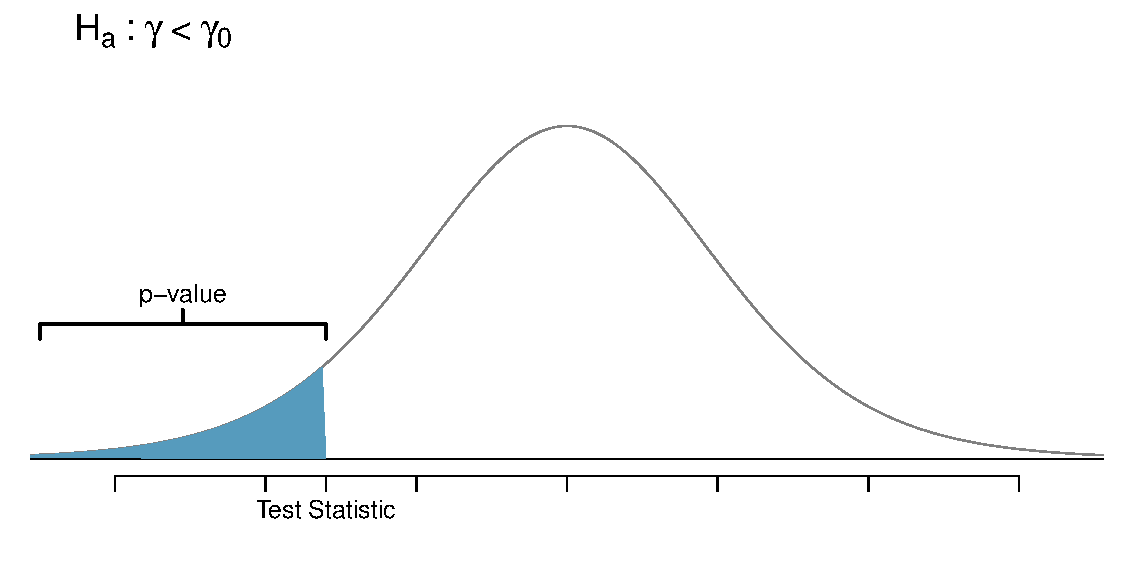
\includegraphics[width=\textwidth]{05-5/figures/pvalAlternateLessThan/pvalAlternateLessThanSmallTail.pdf}
\captionsetup{width=0.9\textwidth}
\caption{Finding the p-value when $H_a : \gamma < \gamma_0$ }
\label{figHaLess}
\end{minipage}
%\hspace{0.5cm}
\quad
\begin{minipage}[b]{0.5\linewidth}
\centering
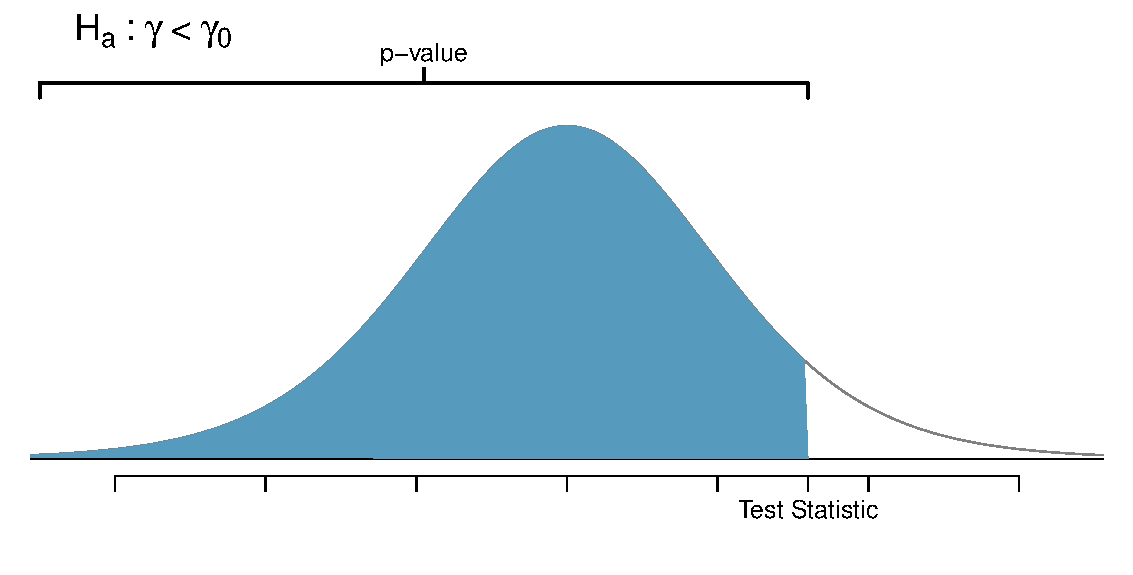
\includegraphics[width=\textwidth]{05-5/figures/pvalAlternateLessThan/pvalAlternateLessThanLargeTail.pdf}
\captionsetup{width=0.9\textwidth}
\caption{Finding the p-value when $H_a : \gamma < \gamma_0$  and we have a large tail}
\label{figHaLessLargeTail}
\end{minipage}
\end{figure}

\begin{caution}
{Finding the p-value for one tailed tests}
{For one tailed tests don't automatically assume that the p-value is the area in the smaller tail.
Refer back to the alternative hypothesis to decide on the area that will give the p-value.}
\end{caution}


When we conduct a two tailed we consider the most extreme cases possible.
This means we look at the area in the tail to the right of $|$test statistic$|$
as well as the area in the tail to the left of -$|$test statistic$|$.
This is illustrated in Figure~\ref{figHaNotEqual}.



\begin{figure}[H]
\centering
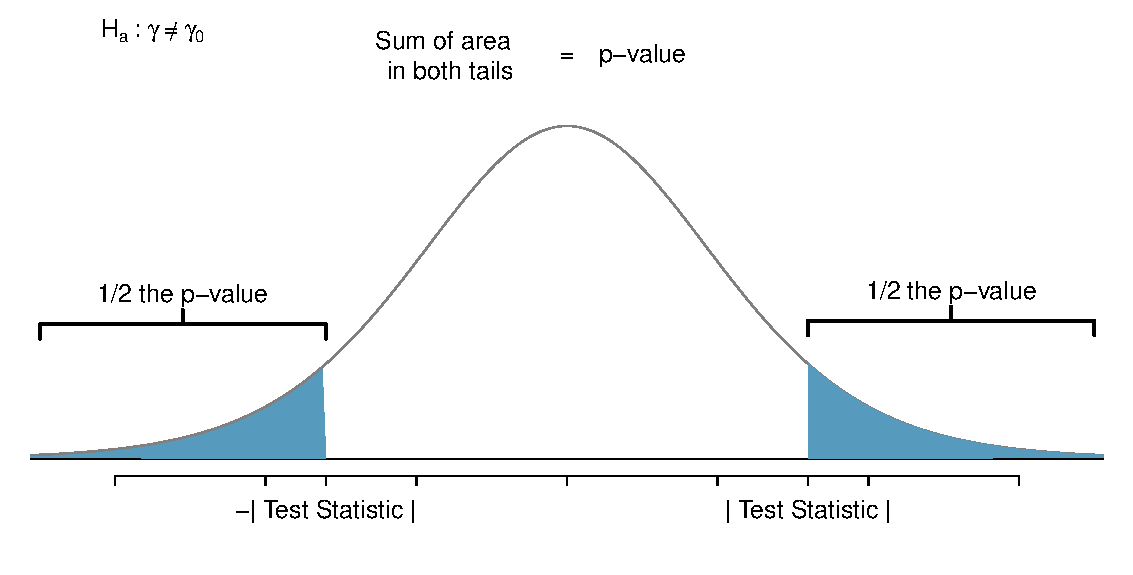
\includegraphics[width=0.85\textwidth]{05-5/figures/pvalTwoTail/pvalTwoTailversion2.pdf}
\captionsetup{width=0.9\textwidth}
\caption{Finding the p-value when $H_a : \gamma \neq \gamma_0$}
\label{figHaNotEqual}
\end{figure}


To find the p-value for a twi tailed test we have to add up the area in both tails.
For symmetric distributions such as the normal and $t$ distribution we can
find the area of one tail and multiply that result by two.

\begin{tipBox}{\tipBoxTitle{Two tailed tests}
When we conduct a two tailed test, make sure that out picture has two tails.
\vspace{0.5mm} }
\end{tipBox}


\begin{tipBox}{\tipBoxTitle{One tailed and two tailed tests}
If the researchers are only interested in showing an increase or a decrease, but not both, use a one tailed test. If the researchers would be interested in any difference from the null value -- an increase or decrease -- then the test should be two tailed.\\
\vspace{0.5mm}}
\end{tipBox}

%Once we calculate a p-value using given sample data and a , it does not change.

%\vfill






\subsection{Compare with a level of significance $\alpha$}

The level of significance is a cut off value (i.e. tolerance) that is used to decide whether we 
should reject the null hypothesis or not.
The level of significance is associated with the symbol $\alpha$.
The p-value is compared with $\alpha$ to determine whether to reject the null hypothesis or not.
The value of $\alpha$ is usually predetermined before conducting a test.
A commonly used value is $\alpha = 0.05$ (which corresponds to a fraction of 1/20).
\footnote{The is the reason we often see the common ``19 times out of 20'' text in articles.}

A natural question to ask is whether we can declare a level of significance for a test 
after we calculate the p-value.
The short answer is that we can, however this is typically not done and it is not considered
a good practice in general since it may give the appearance that results are being
doctored to favour a researchers' beliefs.



\pagebreak 

\subsection{Make a conclusion}

The conclusion we make on our hypothesis test depends on our p-value and $\alpha$.
A summary of the manner in which confusions are made is given below.

\begin{termBox}{\tBoxTitle{Making a conclusion on a hypothesis test}
\hfill\\
\begin{tabular}{lcl}
p-value $> \alpha$	&	$\longrightarrow$	&	The evidence supports the null hypothesis.\\
				&					&	Do not reject the null hypothesis.		\\
\hfill\\
p-value $> \alpha$	&	$\longrightarrow$	&	The evidence is against the null hypothesis.\\
				&					&	The evidence rejects the null hypothesis.
\end{tabular}
}
\index{hypothesis testing!p-value|)}
\end{termBox}

Notice how we use conservative language and state that we do ``not reject the null hypothesis'' or the 
``evidence is against the null hypothesis''.
It is incorrect to state that the ``null hypothesis is wrong'' or ``The null hypothesis is right''.
This kind of language indicates that we are completely certain about the result of a test.
We are working with probabilities so we do not state that our conclusion is completely correct for certain 
since we may have obtained a bad sample that is not representative of the data resulting in 
an incorrect conclusion.
We will learn more about the errors that could occur in a hypothesis test in
{\color{red}{Chapter ???}}.


\begin{termBox}{\tBoxTitle{p-value as a tool in hypothesis testing}
The p-value quantifies how strongly the data favour $H_a$ over $H_0$. 
The smaller the p-value the stronger the evidence against $H_0$.\\

A sufficiently small p-value (usually $<0.05$) corresponds to sufficient evidence to reject $H_0$ in favor of $H_a$.}
\index{hypothesis testing!p-value|)}
\end{termBox}

Another reason that we say we do not ``reject the null hypothesis'' is because 
the evidence we have does not indicate that we definitely have the correct null hypothesis;
it's more to do with the evidence is not at a sufficiently strong level to be against it.
This is similar to a jury making a decision in court.
A person is considered innocent until proven guilty, so a person is considered innocent under the null.
Evidence presented may be circumstantial, however if this evidence may not be strong enough to raise 
enough doubt beyond a reasonable level, the jury should consider the person to be innocent.

Jurors examine the evidence to see whether it convincingly shows a defendant is guilty. Even if the jurors leave unconvinced of guilt beyond a reasonable doubt, this does not mean they believe the defendant is innocent. This is also the case with hypothesis testing: \emph{even if we fail to reject the null hypothesis, we typically do not accept the null hypothesis as true}. Failing to find strong evidence for the alternative hypothesis is not equivalent to accepting the null hypothesis.

\begin{tipBox}{\tipBoxTitle{Hypothesis testing framework}
The skeptic will not reject the null hypothesis ($H_0$), unless the evidence in favor of the alternative hypothesis ($H_a$) is so strong that she rejects $H_0$ in favor of $H_a$.}
\end{tipBox}

Although we make this comparison, a statistical test of hypothesis is usually less subjective than 
circumstantial evidence in a trial.


\vfill

%\begin{tipBox}{\tipBoxTitle{One-sided and two-sided tests}
%If the researchers are only interested in showing an increase or a decrease, but not both, use a one-sided test. If the researchers would be interested in any difference from the null value -- an increase or decrease -- then the test should be two-sided.\vspace{0.5mm}}
%\end{tipBox}


%Unlike the p-value, we can change $\alpha$ since $\alpha$ does not depend on anything.






%\pagebreak 

%\subsection{Hypothesis testing framework}
\hfill\\
\subsection{Testing hypotheses using confidence intervals}
\label{utilizingOurCI}

A simple way to conduct a two-sided hypothesis test is by using a confidence interval. 
To state briefly, the conclusion we make is that the evidence would fail to reject
the null hypothesis of equality at a significance level of $\alpha$ if the hypothesized value
of the parameter under the null hypothesis is inside an approximate $(100-\alpha)\%$ confidence
interval for the parameter (and vice versa if the hypothesized value of the parameter under the null 
hypothesis is not inside the interval).

We will illustrate this procedure with an example.
Is the typical US runner getting faster or slower over time? We consider this question in the context of the Cherry Blossom Run, comparing runners in 2006 and 2012. Technological advances in shoes, training, and diet might suggest runners would be faster in 2012. An opposing viewpoint might say that with the average body mass index on the rise, people tend to run slower. In fact, all of these components might be influencing run time.

In addition to considering run times in this section, we consider a topic near and dear to most students: sleep. A recent study found that college students average about 7 hours of sleep per night.\footnote{\urlwofont{http://theloquitur.com/?p=1161}} However, researchers at a rural college are interested in showing that their students sleep longer than seven hours on average. 
%We investigate this topic in Section~\ref{pValue}.


The average time for all runners who finished the Cherry Blossom Run in 2006 was 93.29 minutes (93 minutes and about 17 seconds). We want to determine if the \data{run10Samp} data set provides strong evidence that the participants in 2012 were faster or slower than those runners in 2006, versus the other possibility that there has been no change.\footnote{While we could answer this question by examining the entire population data (\data{run10}), we only consider the sample data (\data{run10Samp}), which is more realistic since we rarely have access to population data.} We simplify these three options into two competing \termsub{hypotheses}{hypothesis}:
\begin{itemize}
\setlength{\itemsep}{0mm}
\item[$H_0$:] The average 10 mile run time was the same for 2006 and 2012.
\item[$H_a$:] The average 10 mile run time for 2012 was \emph{different} than that of 2006.
\end{itemize}
%We call $H_0$\marginpar[\raggedright\vspace{6mm}

%$H_0$\\\footnotesize null hypothesis\vspace{3mm}\\\normalsize $H_a$\\\footnotesize alternative\\ hypothesis]{\raggedright\vspace{6mm}
%
%$H_0$\\\footnotesize null hypothesis\vspace{3mm}\\\normalsize $H_a$\\\footnotesize alternative\\ hypothesis} the null hypothesis and $H_a$ the alternative hypothesis.

%\begin{termBox}{\tBoxTitle{Null and alternative hypotheses}
%{\small The \term{null hypothesis ($H_0$)} often represents either a skeptical perspective or a claim to be tested. The \term{alternative hypothesis ($H_a$)} represents an alternative claim under consideration and is often represented by a range of possible parameter values.}}
%\end{termBox}



\begin{exercise} \label{hypTestCourtExample}
A US court considers two possible claims about a defendant: she is either innocent or guilty. If we set these claims up in a hypothesis framework, which would be the null hypothesis and which the alternative?\footnote{The jury considers whether the evidence is so convincing (strong) that there is no reasonable doubt regarding the person's guilt; in such a case, the jury rejects innocence (the null hypothesis) and concludes the defendant is guilty (alternative hypothesis).}
\end{exercise}

In the example with the Cherry Blossom Run, the null hypothesis represents no difference in the average time from 2006 to 2012. The alternative hypothesis represents something new or more interesting: there was a difference, either an increase or a decrease. These hypotheses can be described in mathematical notation using $\mu_{12}$ as the average run time for 2012:
\begin{itemize}
\setlength{\itemsep}{0mm}
\item[$H_0$:] $\mu_{12} = 93.29$ %93.28864
\item[$H_a$:] $\mu_{12} \neq 93.29$
\end{itemize}
where $93.29$ minutes (93 minutes and about 17 seconds) is the average 10 mile time for all runners in the 2006 Cherry Blossom Run. Using this mathematical notation, the hypotheses can now be evaluated using statistical tools. We call 93.29 the \term{null value} since it represents the value of the parameter if the null hypothesis is true. We will use the \data{run10Samp} data set to evaluate the hypothesis test.


%\subsection{Testing hypotheses using confidence intervals}
%\label{utilizingOurCI}

We can start the evaluation of the hypothesis setup by comparing 2006 and 2012 run times using a point estimate from the 2012 sample: $\bar{x}_{12} = 95.61$ minutes. This estimate suggests the average time is actually longer than the 2006 time, 93.29 minutes. However, to evaluate whether this provides strong evidence that there has been a change, we must consider the uncertainty associated with $\bar{x}_{12}$.

We learned in Section~\ref{variabilityInEstimates} that there is fluctuation from one sample to another, and it is very unlikely that the sample mean will be exactly equal to our parameter; we should not expect $\bar{x}_{12}$ to exactly equal $\mu_{12}$. Given that $\bar{x}_{12} = 95.61$, it might still be possible that the population average in 2012 has remained unchanged from 2006. The difference between $\bar{x}_{12}$ and 93.29 could be due to \emph{sampling variation}, i.e. the variability associated with the point estimate when we take a random sample.

In Section~\ref{confidenceIntervals}, confidence intervals were introduced as a way to find a range of plausible values for the population mean. 
In Example~\ref{exampleCherryBlossom95CI} using data in
%Based on 
\data{run10Samp}, a 95\% confidence interval for the 2012 population mean, $\mu_{12}$, was calculated as
\begin{eqnarray*}
(92.51, 98.71)
%(92.45, 98.77)
\end{eqnarray*}
Recall that in this example, we knew that the value of $\sigma$ is 1.58 minutes.
Since the 2006 mean of 93.29 falls in the range of plausible values, we cannot say the null hypothesis is implausible. That is, we failed to reject the null hypothesis, $H_0$. 

\begin{tipBox}{\tipBoxTitle{Double negatives can sometimes be used in statistics}
In many statistical explanations, we use double negatives. For instance, we might say that the null hypothesis is \emph{not implausible} or we \emph{failed to reject} the null hypothesis. Double negatives are used to communicate that while we are not rejecting a position, we are also not saying it is correct.}
\end{tipBox}

%\begin{example}{Next consider whether there is strong evidence that the average age of runners has changed from 2006 to 2012 in the Cherry Blossom Run. In 2006, the average age was 36.13 years, and in the 2012 \data{run10Samp} data set, the average was 35.05 years with a standard deviation of 8.97 years for 100 runners.}
\begin{example}{Next consider whether there is strong evidence that the average age of runners has changed from 2006 to 2012 in the Cherry Blossom Run. In 2006, the average age was 36.13 years, and in the 2012 \data{run10Samp} data set, the average was 35.05 years for 100 runners.
Suppose that the standard deviation of all runners is 8.97 years.}
First, set up the hypotheses:
\begin{itemize}
\setlength{\itemsep}{0mm}
\item[$H_0$:] The average age of runners has not changed from 2006 to 2012, $\mu_{age} = 36.13$.
\item[$H_a$:] The average age of runners has changed from 2006 to 2012, $\mu_{age} \neq 36.13$.
\end{itemize}
We have previously verified conditions for this data set. The normal model may be applied to $\bar{y}$ and the estimate of $SE$ should be very accurate. Using the sample mean and standard error, we can construct a 95\% confidence interval for $\mu_{age}$ to determine if there is sufficient evidence to reject $H_0$:
%\begin{eqnarray*}
%\bar{y}\ \pm\ 1.96 \times  \frac{s}{\sqrt{100}} 
%	\quad\to\quad 35.05\ \pm\ 1.96\times 0.90 
%	\quad\to\quad (33.29, 36.81)
%\end{eqnarray*}
\begin{equation*}
\bar{y}\ \pm\ 1.96 \times  \frac{\sigma}{\sqrt{100}}  ~=~ 35.05\ \pm\ 1.96\times 0.90 ~=~ (33.29, 36.81)
\end{equation*}
%\begin{align*}
%\bar{y}\ \pm\ 1.96 \times  \frac{\sigma}{\sqrt{100}} 	& ~=~ 35.05\ \pm\ 1.96\times 0.90 \\
%	& ~=~ (33.29, 36.81)
%\end{align*}
This confidence interval contains the \emph{null value}, 36.13. Because 36.13 is not implausible, we cannot reject the null hypothesis. We have not found strong evidence that the average age is different than 36.13 years.
\index{data!run10Samp|)}
\index{data!run10|)}
\end{example}

\begin{exercise} \label{htForHousingExpenseForCommunityCollege650}
Colleges frequently provide estimates of student expenses such as housing. A consultant hired by a community college claimed that the average student housing expense was \$650 per month. What are the null and alternative hypotheses to test whether this claim is accurate?\footnote{$H_0$: The average cost is \$650 per month, $\mu = \$650$.

\hspace{3.4mm}$H_a$: The average cost is different than \$650 per month, $\mu \neq \$650$.}
\end{exercise}

\begin{exercise} \label{normalDistCondForHousingExpenseForCommunityCollege650}
The community college decides to collect data to evaluate the \$650 per month claim. They take a random sample of 75 students at their school and obtain the data represented in Figure~\ref{communityCollegeClaimedHousingExpenseDistribution}. Can we apply the normal model to the sample mean?\footnote{Applying the normal model requires that certain conditions are met. Because the data are a simple random sample and the sample (presumably) represents no more than 10\% of all students at the college, the observations are independent. The sample size is also sufficiently large ($n=75$) and the data exhibit only moderate skew. Thus, the normal model may be applied to the sample mean.}

\begin{figure}[H]
\centering
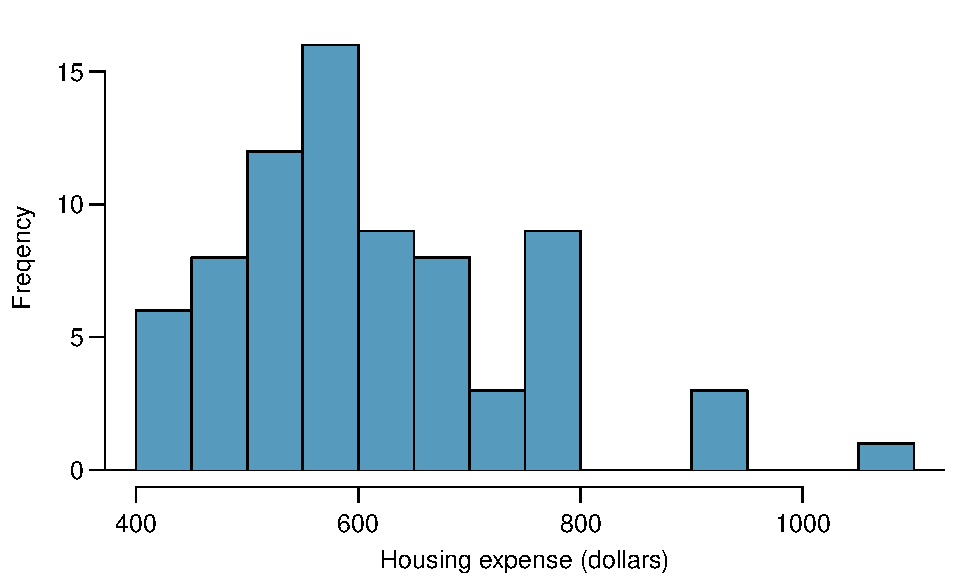
\includegraphics[width=0.75\textwidth]{04/figures/communityCollegeClaimedHousingExpenseDistribution/communityCollegeClaimedHousingExpenseDistribution}
\captionsetup{width=0.9\textwidth}
\caption{Sample distribution of student housing expense. These data are moderately skewed\index{skew!example: moderate}, roughly determined using the outliers on the~right.}
\label{communityCollegeClaimedHousingExpenseDistribution}
\end{figure}
\end{exercise}



\begin{example}{The sample mean for student housing is \$611.63 and the population standard deviation is \$132.85. Construct a 95\% confidence interval for the population mean and evaluate the hypotheses of Exercise~\ref{htForHousingExpenseForCommunityCollege650}.}
The standard error associated with the mean may be estimated using the sample standard deviation divided by the square root of the sample size. Recall that $n=75$ students were sampled.
$$ SE = \frac{\sigma}{\sqrt{n}} = \frac{132.85}{\sqrt{75}} = 15.34 $$
You showed in Exercise~\ref{normalDistCondForHousingExpenseForCommunityCollege650} that the normal model may be applied to the sample mean. This ensures a 95\% confidence interval may be accurately constructed:
%$$\bar{x}\ \pm\ z^{\star} SE \quad\to\quad 611.63\ \pm\ 1.96 \times  15.34 \quad \to \quad (581.56, 641.70) $$
$$\bar{x}\ \pm\ z_{\alpha/2} SE = 611.63\ \pm\ 1.96 \times  15.34 = (581.56, 641.70) $$
Because the null value \$650 is not in the confidence interval, a true mean of \$650 is implausible and we reject the null hypothesis. The data provide statistically significant evidence that the actual average housing expense is less than \$650 per month.
\end{example}








\section{One sample hypothesis tests}

\subsection{On the mean}

\subsubsection{When $\sigma$ is known}

In the case that we know the population standard deviation, the test statistic that is used to perform hypothesis
tests on the mean is:

\begin{termBox}{\tBoxTitle{Test statistic for a hypothesis test on $\mu$ when $\sigma$ is known}
\begin{equation}
Z^{*}	 =   \frac{ \bar{x} - \mu_{0} }{ \sigma / \sqrt{n} }	\label{eqnTestStatSigmaKnown}\\
\end{equation}

Reference distribution:	Standard normal distribution
}
\end{termBox}


%{\huge{ABC}}
%\subsection{Formal testing using p-values}
%\label{pValue}
%
%\index{hypothesis testing!p-value|(}
%
%The p-value is a way of quantifying the strength of the evidence against the null hypothesis and in favor of the alternative. Formally the \emph{p-value} is a conditional probability.
%
%\begin{termBox}{\tBoxTitle{p-value}
%The \term{p-value}\index{hypothesis testing!p-value|textbf} is the probability of observing data at least as favorable to the alternative hypothesis as our current data set, if the null hypothesis is true. We typically use a summary statistic of the data, in this chapter the sample mean, to help compute the p-value and evaluate the hypotheses.}
%\end{termBox}



\index{data!school sleep|(}


%\begin{exercise} \label{skepticalPerspOfRuralSchoolSleepExercise}
%A poll by the National Sleep Foundation found that college students average about 7 hours of sleep per night. Researchers at a rural school are interested in showing that students at their school sleep longer than seven hours on average, and they would like to demonstrate this using a sample of students. What would be an appropriate skeptical position for this research?\footnote{A skeptic would have no reason to believe that sleep patterns at this school are different than the sleep patterns at another school.}
%\end{exercise}

Let's do an example to illustrate all the steps we listed in Chapter~\ref{hypothesisTesting}.
We will work out an example related to 



\subsubsection{When $\sigma$ is not known}

We will examine an example related to sleep.
A poll by the National Sleep Foundation found that college students average about 7 hours of sleep per night. Researchers at a rural school are interested in showing that students at their school sleep longer than seven hours on average, and they would like to demonstrate this using a sample of students. What would be an appropriate skeptical position for this research?

A skeptic would have no reason to believe that sleep patterns at this school are different than the sleep patterns at another school.
We can set up the null hypothesis for this test as a skeptical perspective: the students at this school average 7 hours of sleep per night. The alternative hypothesis takes a new form reflecting the interests of the research: the students average more than 7 hours of sleep. We can write these hypotheses as
\begin{itemize}
\setlength{\itemsep}{0mm}
\item[$H_0$:] $\mu = 7$.
\item[$H_a$:] $\mu > 7$.
\end{itemize}

Since our alternative is $\mu > 7$, we are conduction a one tailed hypothesis test.
 In this investigation, there is no apparent interest in learning whether the mean is less than 7~hours.\footnote{This is entirely based on the interests of the researchers. Had they been only interested in the opposite case -- showing that their students were actually averaging fewer than seven hours of sleep but not interested in showing more than 7 hours -- then our setup would have set the alternative as $\mu < 7$.} 
 %Earlier we encountered a \term{two-sided} hypothesis where we looked for any clear difference, greater than or less than the null value.

%Always use a two-sided test unless it was made clear prior to data collection that the test should be one-sided. Switching a two-sided test to a one-sided test after observing the data is dangerous because it can inflate the Type~1 Error rate. 

%\begin{tipBox}{\tipBoxTitle{One-sided and two-sided tests}
%If the researchers are only interested in showing an increase or a decrease, but not both, use a one-sided test. If the researchers would be interested in any difference from the null value -- an increase or decrease -- then the test should be two-sided.\vspace{0.5mm}}
%\end{tipBox}

%\begin{tipBox}{\tipBoxTitle{Always write the null hypothesis as an equality}
%We will find it most useful if we always list the null hypothesis as an equality (e.g. $\mu = 7$) while the alternative always uses an inequality (e.g. $\mu\neq7$, $\mu>7$, or $\mu<7$).}
%\end{tipBox}

The researchers at the rural school conducted a simple random sample of $n=110$ students on campus. They found that these students averaged 7.42 hours of sleep and the standard deviation of the amount of sleep for the students was 1.75 hours. A histogram of the sample is shown in Figure~\ref{histOfSleepForCollegeThatWasCheckingForMoreThan7Hours}.

\begin{figure}
\centering
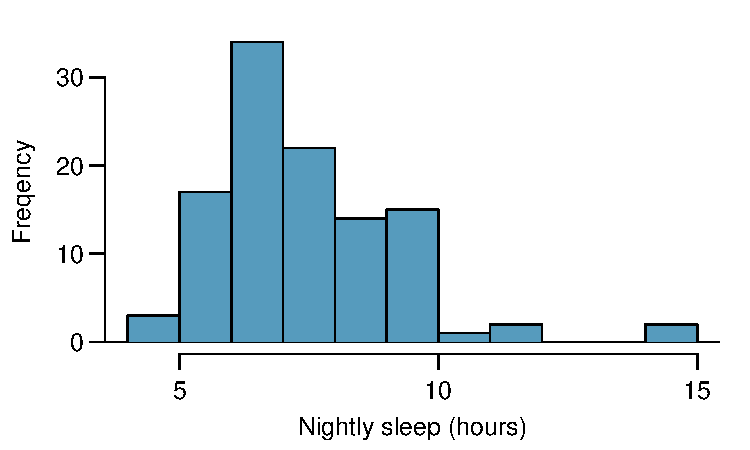
\includegraphics[height=55mm]{04/figures/histOfSleepForCollegeThatWasCheckingForMoreThan7Hours/histOfSleepForCollegeThatWasCheckingForMoreThan7Hours}
\caption{Distribution of a night of sleep for 110 college students. These data are moderately skewed.\index{skew!example: moderate}}
\label{histOfSleepForCollegeThatWasCheckingForMoreThan7Hours}
\end{figure}

Before we can use a normal model for the sample mean or compute the standard error of the sample mean, we must verify conditions. (1)~Because this is a simple random sample from less than 10\% of the student body, the observations are independent. (2)~The sample size in the sleep study is sufficiently large since it is greater than 30. (3)~The data show moderate skew in Figure~\ref{histOfSleepForCollegeThatWasCheckingForMoreThan7Hours} and the presence of a couple of outliers. This skew and the outliers (which are not too extreme) are acceptable for a sample size of $n=110$. With these conditions verified, the normal model can be safely applied to $\bar{x}$ and the estimated standard error will be very accurate.

\begin{exercise} \label{findSEOfFirstSleepStudyCheckingGreaterThan7Hours}
What is the standard deviation associated with $\bar{x}$? That is, estimate the standard error of $\bar{x}$.\footnote{The standard error can be estimated from the sample standard deviation and the sample size: $SE_{\bar{x}} = \frac{s_x}{\sqrt{n}} = \frac{1.75}{\sqrt{110}} = 0.17$.}
\end{exercise}

The hypothesis test will be evaluated using a significance level of $\alpha = 0.05$. We want to consider the data under the scenario that the null hypothesis is true. In this case, the sample mean is from a distribution that is nearly normal and has mean 7 and standard deviation of about 0.17. Such a distribution is shown in Figure~\ref{pValueOneSidedSleepStudy}.

\begin{figure}[H]
   \centering
   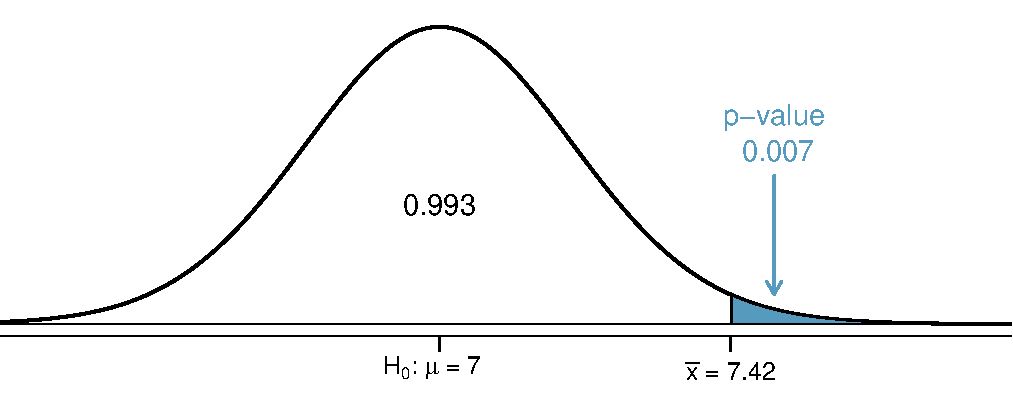
\includegraphics[width=0.73\textwidth]{04/figures/pValueOneSidedSleepStudy/pValueOneSidedSleepStudy}
   \caption{If the null hypothesis is true, then the sample mean $\bar{x}$ came from this nearly normal distribution. The right tail describes the probability of observing such a large sample mean if the null hypothesis is true.}
   \label{pValueOneSidedSleepStudy}
\end{figure}

The shaded tail in Figure~\ref{pValueOneSidedSleepStudy} represents the chance of observing such a large mean, conditional on the null hypothesis being true. That is, the shaded tail represents the p-value. We shade all means larger than our sample mean, $\bar{x} = 7.42$, because they are more favorable to the alternative hypothesis than the observed mean.

We compute the p-value by finding the tail area of this normal distribution, which we learned to do in Section~\ref{normalDist}. First compute the Z score of the sample mean, $\bar{x} = 7.42$:
\begin{eqnarray*}
Z = \frac{\bar{x} - \text{null value}}{SE_{\bar{x}}} = \frac{7.42 - 7}{0.17} = 2.47
\end{eqnarray*}
Using the normal probability table, the lower unshaded area is found to be 0.993. Thus the shaded area is $1-0.993 = 0.007$. {\em If the null hypothesis is true, the probability of observing such a large sample mean for a sample of 110 students is only 0.007.}\index{p-value!interpretation example} That is, if the null hypothesis is true, we would not often see such a large mean.

We evaluate the hypotheses by comparing the p-value to the significance level. Because the p-value is less than the significance level (p-value $=0.007 < 0.05=\alpha$), we reject the null hypothesis. What we observed is so unusual with respect to the null hypothesis that it casts serious doubt on $H_0$ and provides strong evidence favoring $H_a$.

%\begin{termBox}{\tBoxTitle{p-value as a tool in hypothesis testing}
%The p-value quantifies how strongly the data favor $H_a$ over $H_0$. A small p-value (usually $<0.05$) corresponds to sufficient evidence to reject $H_0$ in favor of $H_a$.}
%\index{hypothesis testing!p-value|)}
%\end{termBox}

\begin{tipBox}{\tipBoxTitle{It is useful to first draw a picture to find the p-value}
It is useful to draw a picture of the distribution of $\bar{x}$ as though $H_0$ was true (i.e. $\mu$ equals the null value), and shade the region (or regions) of sample means that are at least as favorable to the alternative hypothesis. These shaded regions represent the p-value.}
\end{tipBox}

The ideas below review the process of evaluating hypothesis tests with p-values:
\begin{itemize}
\setlength{\itemsep}{0mm}
\item The null hypothesis represents a skeptic's position or a position of no difference. We reject this position only if the evidence strongly favors $H_a$.
\item A small p-value means that if the null hypothesis is true, there is a low probability of seeing a point estimate at least as extreme as the one we saw. We interpret this as strong evidence in favor of the alternative.
\item We reject the null hypothesis if the p-value is smaller than the significance level, $\alpha$, which is usually 0.05. Otherwise, we fail to reject $H_0$.
\item We should always state the conclusion of the hypothesis test in plain language so non-statisticians can also understand the results.
\end{itemize}

The p-value is constructed in such a way that we can directly compare it to the significance level ($\alpha$) to determine whether or not to reject $H_0$. This method ensures that the Type~1 Error rate does not exceed the significance level standard. 












\vfill












\pagebreak


\section{Decision errors}

\index{hypothesis testing!decision errors|(}

Hypothesis tests are not flawless. Just think of the court system: innocent people are sometimes wrongly convicted and the guilty sometimes walk free. Similarly, we can make a wrong decision in statistical hypothesis tests. However, the difference is that we have the tools necessary to quantify how often we make such errors.

There are two competing hypotheses: the null and the alternative. In a hypothesis test, we make a statement about which one might be true, but we might choose incorrectly. There are four possible scenarios in a hypothesis test, which are summarized in Table~\ref{fourHTScenarios}.

\begin{table}[ht]
\centering
\begin{tabular}{l l c c}
& & \multicolumn{2}{c}{\textbf{Test conclusion}} \\
  \cline{3-4}
\vspace{-3.7mm} \\
& & do not reject $H_0$ &  reject $H_0$ in favor of $H_a$ \\
  \cline{2-4}
\vspace{-3.7mm} \\
& $H_0$ true & okay &  Type~1 Error \\
\raisebox{1.5ex}{\textbf{Truth}} & $H_a$ true & Type 2 Error & okay \\
  \cline{2-4}
\end{tabular}
\caption{Four different scenarios for hypothesis tests.}
\label{fourHTScenarios}
\end{table}

A \term{Type~1 Error} is rejecting the null hypothesis when $H_0$ is actually true. A \term{Type~2 Error} is failing to reject the null hypothesis when the alternative is actually true.

\begin{exercise} \label{whatAreTheErrorTypesInUSCourts}
In a US court, the defendant is either innocent ($H_0$) or  guilty ($H_a$). What does a Type~1 Error represent in this context? What does a Type 2 Error represent? Table~\ref{fourHTScenarios} may be useful.\footnote{If the court makes a Type~1 Error, this means the defendant is innocent ($H_0$ true) but wrongly convicted. A Type 2 Error means the court failed to reject $H_0$ (i.e. failed to convict the person) when she was in fact guilty ($H_a$ true).}
\end{exercise}

\begin{exercise} \label{howToReduceType1ErrorsInUSCourts}
How could we reduce the Type~1 Error rate in US courts? What influence would this have on the Type 2 Error rate?\footnote{To lower the Type~1 Error rate, we might raise our standard for conviction from ``beyond a reasonable doubt'' to ``beyond a conceivable doubt'' so fewer people would be wrongly convicted. However, this would also make it more difficult to convict the people who are actually guilty, so we would make more Type~2 Errors.}
\end{exercise}

\begin{exercise} \label{howToReduceType2ErrorsInUSCourts}
How could we reduce the Type~2 Error rate in US courts? What influence would this have on the Type~1 Error rate?\footnote{To lower the Type~2 Error rate, we want to convict more guilty people. We could lower the standards for conviction from ``beyond a reasonable doubt'' to ``beyond a little doubt''. Lowering the bar for guilt will also result in more wrongful convictions, raising the Type~1 Error rate.}
\end{exercise}

\index{hypothesis testing!decision errors|)}

Exercises~\ref{whatAreTheErrorTypesInUSCourts}-\ref{howToReduceType2ErrorsInUSCourts} provide an important lesson: if we reduce how often we make one type of error, we generally make more of the other type.

Hypothesis testing is built around rejecting or failing to reject the null hypothesis. That is, we do not reject $H_0$ unless we have strong evidence. But what precisely does \emph{strong evidence} mean? As a general rule of thumb, for those cases where the null hypothesis is actually true, we do not want to incorrectly reject $H_0$ more than 5\% of the time. This corresponds to a \term{significance level}\index{hypothesis testing!significance level} of 0.05. We often write the significance level using $\alpha$\marginpar[\raggedright\vspace{-4mm}

$\alpha$\\\footnotesize significance\\level of a\\hypothesis test]{\raggedright\vspace{-4mm}

$\alpha$\\\footnotesize significance\\level of a\\hypothesis test} (the Greek letter \emph{alpha}\index{Greek!alpha@alpha ($\alpha$)}): $\alpha = 0.05$. We discuss the appropriateness of different significance levels in Section~\ref{significanceLevel}.

If we use a 95\% confidence interval to test a hypothesis where the null hypothesis is true, we will make an error whenever the point estimate is at least 1.96 standard errors away from the population parameter. This happens about 5\% of the time (2.5\% in each tail). Similarly, using a 99\% confidence interval to evaluate a hypothesis is equivalent to a significance level of $\alpha = 0.01$.

A confidence interval is, in one sense, simplistic in the world of hypothesis tests. Consider the following two scenarios:
\begin{itemize}
\setlength{\itemsep}{0mm}
\item The null value (the parameter value under the null hypothesis) is in the 95\% confidence interval but just barely, so we would not reject $H_0$. However, we might like to somehow say, quantitatively, that it was a close decision.
\item The null value is very far outside of the interval, so we reject $H_0$. However, we want to communicate that, not only did we reject the null hypothesis, but it wasn't even close. Such a case is depicted in Figure~\ref{whyWeWantPValue}.
\end{itemize}
%In Section~\ref{pValue}, we introduce a tool called the \emph{p-value} that will be helpful in these cases. The p-value method also extends to hypothesis tests where confidence intervals cannot be easily constructed or applied.

\begin{figure}[H]
\centering
\captionsetup{width=0.9\textwidth}
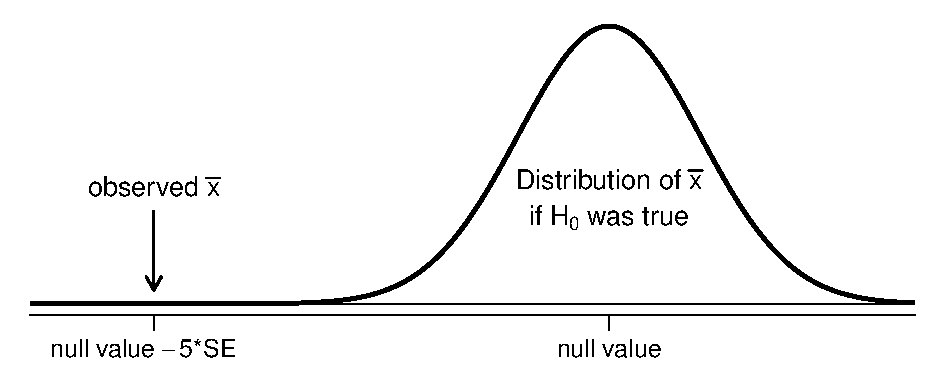
\includegraphics[width=0.75\textwidth]{04/figures/whyWeWantPValue/whyWeWantPValue}
\caption{It would be helpful to quantify the strength of the evidence against the null hypothesis. In this case, the evidence is extremely strong.
This figure is illustrative of the reason we use p-values.}
\label{whyWeWantPValue}
\end{figure}










\pagebreak

\begin{figure}[H]
   \centering
   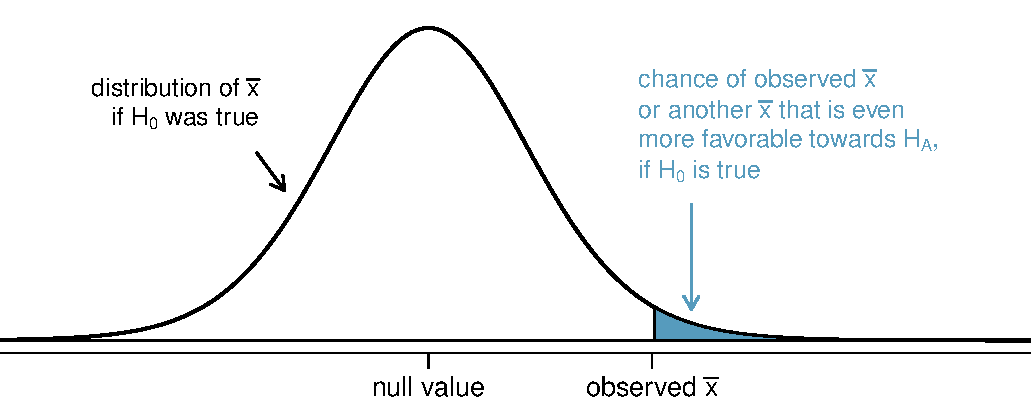
\includegraphics[width=0.9\textwidth]{04/figures/pValueOneSidedSleepStudyExplained/pValueOneSidedSleepStudyExplained}
   \caption{To identify the p-value, the distribution of the sample mean is considered as if the null hypothesis was true. Then the p-value is defined and computed as the probability of the observed $\bar{x}$ or an $\bar{x}$ even more favorable to $H_a$ under this distribution.}
   \label{pValueOneSidedSleepStudyExplained}
\end{figure}


\pagebreak


\pagebreak

\begin{exercise}
If the null hypothesis is true, how often should the p-value be less than 0.05?\footnote{About 5\% of the time. If the null hypothesis is true, then the data only has a 5\% chance of being in the 5\% of data most favorable to $H_a$.}
\index{data!school sleep|)}
\end{exercise}

\begin{exercise}
Suppose we had used a significance level of 0.01 in the sleep study. Would the evidence have been strong enough to reject the null hypothesis? (The p-value was 0.007.) What if the significance level was $\alpha = 0.001$? \footnote{We reject the null hypothesis whenever $p$-$value < \alpha$. Thus, we would still reject the null hypothesis if $\alpha = 0.01$ but not if the significance level had been $\alpha = 0.001$.}
\end{exercise}

\begin{exercise} \label{ebayAmazonOneSidedTestExercise}
\index{data!mario\_kart|(}
Ebay might be interested in showing that buyers on its site tend to pay less than they would for the corresponding new item on Amazon. We'll research this topic for one particular product: a video game called \emph{Mario Kart} for the Nintendo Wii. During early October 2009, Amazon sold this game for \$46.99. Set up an appropriate (one-sided!) hypothesis test to check the claim that Ebay buyers pay less during auctions at this same time.\footnote{The skeptic would say the average is the same on Ebay, and we are interested in showing the average price is lower.
\begin{itemize}
\setlength{\itemsep}{0mm}
\item[$H_0$:] The average auction price on Ebay is equal to (or more than) the price on Amazon. We write only the equality in the statistical notation: $\mu_{ebay} = 46.99$.
\item[$H_a$:] The average price on Ebay is less than the price on Amazon, $\mu_{ebay} < 46.99$.
\end{itemize}}
\end{exercise}


\begin{exercise} \label
{exerciseFor52EbayAuctionsToExamineMarioKartLessExpensiveThanAmazonConditions}
During early October, 2009, 52 Ebay auctions were recorded for \emph{Mario Kart}.\footnote{These data were collected by OpenIntro staff.} The total prices for the auctions are presented using a histogram in Figure~\ref{ebayMarioKartAuctionPriceHistogramFor3ConditionsExercise}, and we may like to apply the normal model to the sample mean. Check the three conditions required for applying the normal model: (1)~independence, (2)~at~least 30 observations, and (3)~the data are not strongly skewed.\footnote{(1) The independence condition is unclear. \emph{We will make the assumption that the observations are independent, which we should report with any final results.} (2) The sample size is sufficiently large: $n =52 \geq 30$. (3) The data distribution is not strongly skewed; it is approximately symmetric.}
\end{exercise}

\begin{figure}
   \centering
   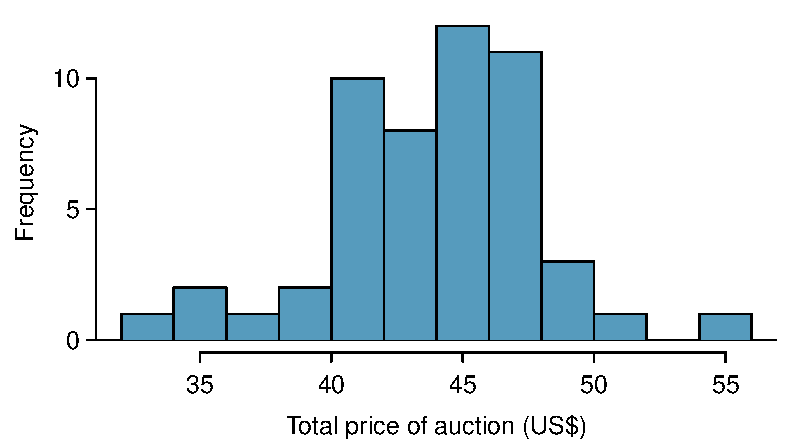
\includegraphics[width=0.68\textwidth]{04/figures/ebayMarioKartAuctionPriceHistogramFor3ConditionsExercise/ebayMarioKartAuctionPriceHistogramFor3ConditionsExercise}
   \caption{A histogram of the total auction prices for 52 Ebay auctions.}
   \label{ebayMarioKartAuctionPriceHistogramFor3ConditionsExercise}
\end{figure}

\begin{example}{The average sale price of the 52 Ebay auctions for \emph{Wii Mario Kart} was \$44.17 with a standard deviation of \$4.15. Does this provide sufficient evidence to reject the null hypothesis in Exercise~\ref{ebayAmazonOneSidedTestExercise}? Use a significance level of $\alpha = 0.01$.}
The hypotheses were set up and the conditions were checked in Exercises~\ref{ebayAmazonOneSidedTestExercise} and~\ref{exerciseFor52EbayAuctionsToExamineMarioKartLessExpensiveThanAmazonConditions}. The next step is to find the standard error of the sample mean and produce a sketch to help find the p-value.
\begin{eqnarray*}
SE_{\bar{x}} = s/\sqrt{n} = 4.15/\sqrt{52} = 0.5755
\end{eqnarray*}
\begin{center}
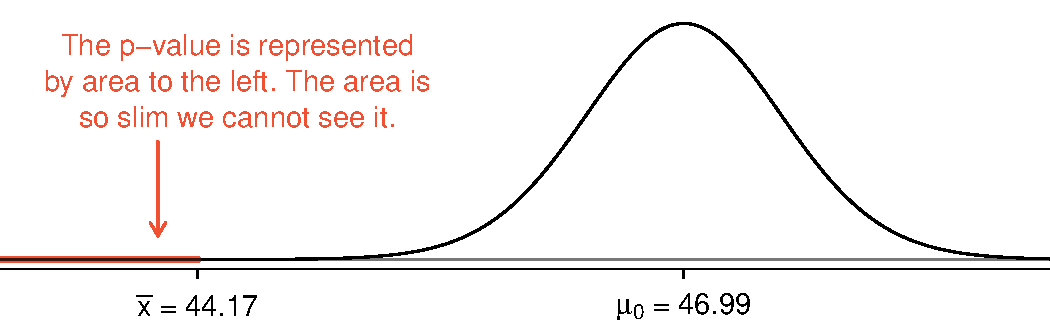
\includegraphics[height=35mm]{04/figures/pVForEbayAmazonComparison/pVForEbayAmazonComparison}
\end{center}
Because the alternative hypothesis says we are looking for a smaller mean, we shade the lower tail. We find this shaded area by using the Z score and normal probability table: $Z = \frac{44.17 - 46.99}{0.5755} = -4.90$, which has area less than 0.0002. The area is so small we cannot really see it on the picture. This lower tail area corresponds to the p-value.

Because the p-value is so small -- specifically, smaller than $\alpha = 0.01$ -- this provides sufficiently strong evidence to reject the null hypothesis in favor of the alternative. The data provide statistically significant evidence that the average price on Ebay is lower than Amazon's asking price.
\index{data!mario\_kart|)}
\end{example}



\pagebreak

\subsection{Two-sided hypothesis testing with p-values}
\label{twoSidedTestsWithPValues}

\index{data!school sleep|(}

We now consider how to compute a p-value for a two-sided test. In one-sided tests, we shade the single tail in the direction of the alternative hypothesis. For example, when the alternative had the form $\mu > 7$, then the p-value was represented by the upper tail (Figure~\ref{pValueOneSidedSleepStudyExplained}). When the alternative was $\mu < 46.99$, the p-value was the lower tail (Exercise~\ref{ebayAmazonOneSidedTestExercise}). In a two-sided test, \emph{we shade two tails} since evidence in either direction is favorable to $H_a$.

\begin{exercise} \label{2ndSchSleepHypSetupExercise}
Earlier we talked about a research group investigating whether the students at their school slept longer than 7 hours each night. Let's consider a second group of researchers who want to evaluate whether the students at their college differ from the norm of 7 hours. Write the null and alternative hypotheses for this investigation.\footnote{Because the researchers are interested in any difference, they should use a two-sided setup: $H_0: \mu = 7$, $H_a: \mu \neq 7$.}
\end{exercise}

\begin{example}{The second college randomly samples 72 students and finds a mean of $\bar{x} = 6.83$ hours and a standard deviation of $s=1.8$ hours. Does this provide strong evidence against $H_0$ in Exercise~\ref{2ndSchSleepHypSetupExercise}? Use a significance level of $\alpha=0.05$.}
First, we must verify assumptions. (1) A simple random sample of less than 10\% of the student body means the observations are independent. (2) The sample size is 72, which is greater than 30. (3) Based on the earlier distribution and what we already know about college student sleep habits, the distribution is probably not strongly~skewed.

Next we can compute the standard error ($SE_{\bar{x}} = \frac{s}{\sqrt{n}} = 0.21$) of the estimate and create a picture to represent the p-value, shown in Figure~\ref{2ndSchSleepHTExample}. Both tails are shaded. An estimate of 7.17 or more provides at least as strong of evidence against the null hypothesis and in favor of the alternative as the observed estimate, $\bar{x} = 6.83$.

We can calculate the tail areas by first finding the lower tail corresponding to $\bar{x}$:
\begin{eqnarray*}
Z = \frac{6.83 - 7.00}{0.21} = -0.81 \quad\stackrel{table}{\rightarrow}\quad \text{left tail}=0.2090
\end{eqnarray*}
Because the normal model is symmetric, the right tail will have the same area as the left tail. The p-value is found as the sum of the two shaded tails:
\begin{eqnarray*}
\text{p-value} = \text{left tail} + \text{right tail} = 2\times(\text{left tail}) = 0.4180
\end{eqnarray*}
This p-value is relatively large (larger than $\alpha=0.05$), so we should not reject $H_0$. That is, if $H_0$ is true, it would not be very unusual to see a sample mean this far from 7 hours simply due to sampling variation. Thus, we do not have sufficient evidence to conclude that the mean is different than 7 hours.

\index{data!school sleep|)}

\begin{figure}
   \centering
   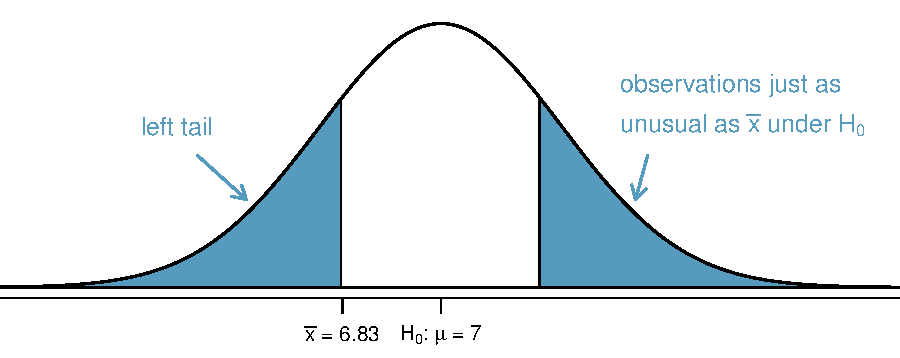
\includegraphics[width=0.9\textwidth]{04/figures/2ndSchSleepHTExample/2ndSchSleepHTExample}
   \caption{$H_a$ is two-sided, so \emph{both} tails must be counted for the p-value.}
   \label{2ndSchSleepHTExample}
\end{figure}

\end{example}

\begin{example}{It is never okay to change two-sided tests to one-sided tests after observing the data. In this example we explore the consequences of ignoring this advice. Using $\alpha=0.05$, we show that freely switching from two-sided tests to one-sided tests will cause us to make twice as many Type~1 Errors as intended.} \label{swappingHypAfterDataDoublesType1ErrorRate}
Suppose the sample mean was larger than the null value, $\mu_0$ (e.g. $\mu_0$ would represent~7 if $H_0$:~$\mu = 7$). Then if we can flip to a one-sided test, we would use $H_a$: $\mu > \mu_0$. Now if we obtain any observation with a Z score greater than 1.65, we would reject $H_0$. If the null hypothesis is true, we incorrectly reject the null hypothesis about 5\% of the time when the sample mean is above the null value, as shown in Figure~\ref{type1ErrorDoublingExampleFigure}.

Suppose the sample mean was smaller than the null value. Then if we change to a one-sided test, we would use $H_a$: $\mu < \mu_0$. If $\bar{x}$ had a Z score smaller than -1.65, we would reject $H_0$. If the null hypothesis is true, then we would observe such a case about 5\% of the time.

By examining these two scenarios, we can determine that we will make a Type~1 Error $5\%+5\%=10\%$ of the time if we are allowed to swap to the ``best'' one-sided test for the data. This is twice the error rate we prescribed with our significance level: $\alpha=0.05$ (!).

\begin{figure}
   \centering
   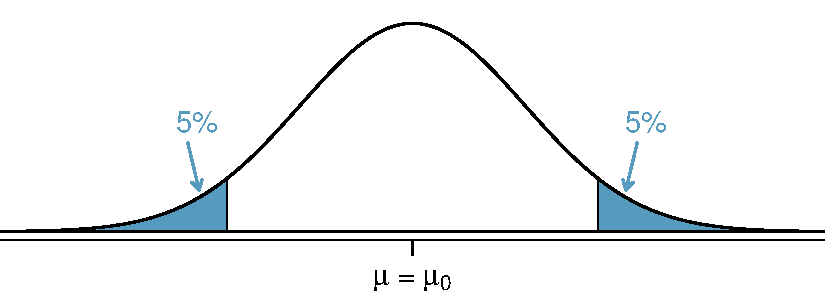
\includegraphics[width=0.7\textwidth]{04/figures/type1ErrorDoublingExampleFigure/type1ErrorDoublingExampleFigure}
   \caption{The shaded regions represent areas where we would reject $H_0$ under the bad practices considered in Example~\ref{swappingHypAfterDataDoublesType1ErrorRate} when $\alpha = 0.05$.}
   \label{type1ErrorDoublingExampleFigure}
\end{figure}

\end{example}

\begin{caution}{One-sided hypotheses are allowed only \emph{before} seeing data}
{After observing data, it is tempting to turn a two-sided test into a one-sided test. Avoid this temptation. Hypotheses must be set up \emph{before} observing the data. If~they are not, the test must be two-sided.}
\end{caution}

\section{Choosing a significance level (special topic)}
\label{significanceLevel}

\index{hypothesis testing!significance level|(}
\index{significance level|(}

Choosing a significance level for a test is important in many contexts, and the traditional level is 0.05. However, it is often helpful to adjust the significance level based on the application. We may select a level that is smaller or larger than 0.05 depending on the consequences of any conclusions reached from the test.

If making a Type~1 Error is dangerous or especially costly, we should choose a small significance level (e.g. 0.01). Under this scenario we want to be very cautious about rejecting the null hypothesis, so we demand very strong evidence favoring $H_a$ before we would reject $H_0$.

If a Type 2 Error is relatively more dangerous or much more costly than a Type~1 Error, then we should choose a higher significance level (e.g. 0.10). Here we want to be cautious about failing to reject $H_0$ when the null is actually false.  We will discuss this particular case in greater detail in Section~\ref{sampleSizeAndPower}.

\begin{tipBox}{\tipBoxTitle[]{Significance levels should reflect consequences of errors}
The significance level selected for a test should reflect the consequences associated with Type~1 and Type 2 Errors.}
\end{tipBox}

\begin{example}{A car manufacturer is considering a higher quality but more expensive supplier for window parts in its vehicles. They sample a number of parts from their current supplier and also parts from the new supplier. They decide that if the high quality parts will last more than 12\% longer, it makes financial sense to switch to this more expensive supplier. Is there good reason to modify the significance level in such a hypothesis test?}
The null hypothesis is that the more expensive parts last no more than 12\% longer while the alternative is that they do last more than 12\% longer. This decision is just one of the many regular factors that have a marginal impact on the car and company. A significance level of 0.05 seems reasonable since neither a Type~1 or Type 2 error should be dangerous or (relatively) much more expensive.
\end{example}

\begin{example}{The same car manufacturer is considering a slightly more expensive supplier for parts related to safety, not windows. If the durability of these safety components is shown to be better than the current supplier, they will switch manufacturers. Is there good reason to modify the significance level in such an evaluation?}
The null hypothesis would be that the suppliers' parts are equally reliable. Because safety is involved, the car company should be eager to switch to the slightly more expensive manufacturer (reject $H_0$) even if the evidence of increased safety is only moderately strong. A slightly larger significance level, such as $\alpha=0.10$, might be appropriate.
\end{example}

\begin{exercise}
A part inside of a machine is very expensive to replace. However, the machine usually functions properly even if this part is broken, so the part is replaced only if we are extremely certain it is broken based on a series of measurements. Identify appropriate hypotheses for this test (in plain language) and suggest an appropriate significance level.\footnote{Here the null hypothesis is that the part is not broken, and the alternative is that it is broken. If we don't have sufficient evidence to reject $H_0$, we would not replace the part. It sounds like failing to fix the part if it is broken ($H_0$ false, $H_a$ true) is not very problematic, and replacing the part is expensive. Thus, we should require very strong evidence against $H_0$ before we replace the part. Choose a small significance level, such as $\alpha=0.01$.}
\end{exercise}

\index{significance level|)}
\index{hypothesis testing!significance level|)}
\index{hypothesis testing|)}
